\documentclass[tikz,border=8pt]{standalone}
\usetikzlibrary{arrows.meta,positioning,fit,calc}
\begin{document}
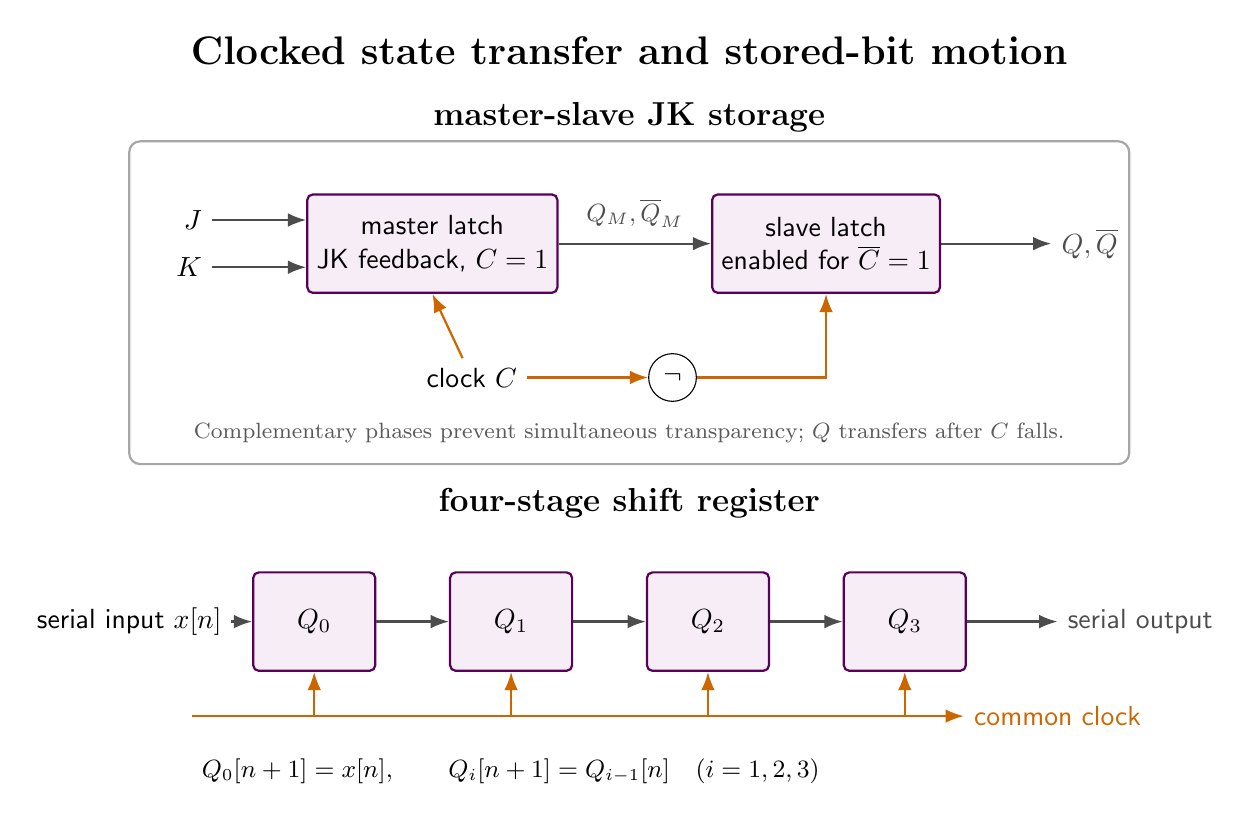
\begin{tikzpicture}[
  font=\sffamily,
  >=Latex,
  block/.style={draw=blue!65!black,rounded corners=2pt,thick,minimum width=2.35cm,minimum height=1.25cm,align=center,fill=blue!6},
  store/.style={block,draw=violet!70!black,fill=violet!7},
  line/.style={->,thick,black!70},
  clock/.style={->,thick,orange!80!black}
]
\node[font=\bfseries\Large] at (7.0,8.7) {Clocked state transfer and stored-bit motion};

% Master-slave pair: complementary enable phases prevent transparency through both stages.
\node[font=\bfseries\large] at (7.0,7.85) {master-slave JK storage};
\node[store] (master) at (4.5,6.25) {master latch\\JK feedback, $C=1$};
\node[store] (slave) at (9.5,6.25) {slave latch\\enabled for $\overline C=1$};
\node[left=1.2cm of master,yshift=.30cm] (j) {$J$};
\node[left=1.2cm of master,yshift=-.30cm] (k) {$K$};
\draw[line] (j) -- ([yshift=.3cm]master.west);
\draw[line] (k) -- ([yshift=-.3cm]master.west);
\draw[line] (master) -- node[above,yshift=2pt,font=\small] {$Q_M,\overline Q_M$} (slave);
\draw[line] (slave.east) -- ++(1.4,0) node[right] {$Q,\overline Q$};
\node (clk) at (5.0,4.55) {clock $C$};
\draw[clock] (clk) -- (master.south);
\node[draw,circle,minimum size=.42cm] (inv) at (7.55,4.55) {$\neg$};
\draw[clock] (clk.east) -- (inv.west);
\draw[clock] (inv.east) -| (slave.south);
\node[font=\footnotesize,text=black!65] at (7.0,3.85)
  {Complementary phases prevent simultaneous transparency; $Q$ transfers after $C$ falls.};
\draw[rounded corners=4pt,thick,black!35] (.65,3.45) rectangle (13.35,7.55);

% Four-stage shift register and its exact recurrence.
\node[font=\bfseries\large] at (7.0,2.95) {four-stage shift register};
\node (sin) at (.65,1.45) {serial input $x[n]$};
\foreach \i/\x in {0/3.0,1/5.5,2/8.0,3/10.5}{
  \node[store,minimum width=1.55cm] (q\i) at (\x,1.45) {$Q_\i$};
}
\draw[line] (sin) -- (q0);
\draw[line] (q0) -- (q1);
\draw[line] (q1) -- (q2);
\draw[line] (q2) -- (q3);
\draw[line] (q3.east) -- ++(1.15,0) node[right] {serial output};
\draw[clock] (1.45,.25) -- (11.25,.25) node[right] {common clock};
\foreach \i in {0,1,2,3}{\draw[clock] (q\i.south |- 1.45,.25) -- (q\i.south);}
\node[font=\small,anchor=west] at (1.45,-.45)
  {$Q_0[n+1]=x[n],\qquad Q_i[n+1]=Q_{i-1}[n]\quad(i=1,2,3)$};
\end{tikzpicture}
\end{document}
